\section{Numerical study}\label{sec:study}

\subsection{Design}

Six target distributions were chosen to exercise different geometries: the
\textbf{normal} (symmetric, unbounded), the \textbf{Gumbel} (right-skewed,
exponential right tail), the \textbf{uniform} (compact support, no mode), the
\textbf{Student-$t$} with $\nu = 4$ degrees of freedom (symmetric, polynomial
tails), the \textbf{Gamma} with shape $2$ (right-skewed, bounded on the left, with
a density that rises linearly from zero) and the \textbf{Beta}$(2, 5)$ (bounded
on both sides and asymmetric). The Student-$t$ is deliberately placed on the
edge of what four-moment matching can do: its tails decay like $|x|^{-5}$, which
corresponds to the shape value $\lambda = -1/4$ at which the fourth moment of the
GLD ceases to exist, and its own kurtosis is infinite. For each target, samples of
size $N \in \{50;\, 200;\, 1{,}000;\, 5{,}000\}$ were drawn and fitted by moment
matching with $15$ multi-start attempts, under both parameterizations. Each cell
was replicated $100$ times with independent samples, giving
$2 \times 6 \times 4 \times 100 = 4{,}800$ fits.

The seed of a replicate is drawn from a seed sequence keyed by the target, $N$
and the replicate index, but not by the parameterization, so FKML and RS are
fitted to \emph{identical} samples. The comparison between them is therefore
paired, and any difference is a property of the parameterization rather than of
the draw.

\subsection{Metrics}

The primary metric is computed against the \emph{analytical} target, not against
a sample, so that it measures the approximation error of the family itself rather
than the noise of a reference draw. Parameterising by $u$ turns the
Kolmogorov-Smirnov distance into a form that needs no root finding,
\begin{equation}
    \mathrm{KS} = \sup_{x} \bigl| F_{\mathrm{GLD}}(x) - F_{\mathrm{target}}(x) \bigr|
                = \sup_{0<u<1} \bigl| u - F_{\mathrm{target}}(Q(u)) \bigr|,
    \label{eq:ks}
\end{equation}
evaluated on a grid of $4{,}001$ probabilities, augmented by the two terms that
account for the mass the target places outside a compact GLD support, where
$F_{\mathrm{GLD}}$ is pinned at $0$ or $1$.

Alongside it we report the sample-based metrics a practitioner can actually
compute, from a reference sample of the target and a sample of the fitted GLD,
both of size $\max(N, 20{,}000)$ and both drawn without tail trimming: the
Kullback-Leibler divergence $D(p \,\|\, q)$ of the target density $p$ from the
fitted density $q$, the Wasserstein distance, and quantile errors at $P_5$,
$P_{50}$ and $P_{95}$ normalised by the distance between the $P_5$ and $P_{95}$
of the target. The divergence is computed between Gaussian kernel density
estimates on a grid that spans the reference sample, with a small floor on the
densities. When the fitted GLD has compact support and the target does not, the
exact $D(p \,\|\, q)$ is infinite; the smoothed estimate stays finite and should
be read as a comparison of the bulk of the two densities, not of their extreme
tails, which the KS distance and the quantile errors cover.

A goodness-of-fit test is also reported, run at the sample size actually
available, $N$ against $N$. Against a large reference sample the two-sample test
asks whether the GLD \emph{is} the target; it is not, so the test rejects
essentially always and its $p$-value carries no information. At size $N$ it asks
the question a practitioner asks of their own data.

Every metric is summarised over the $100$ replicates of a cell by its median,
and the KS distance also by its interquartile range (IQR).

\subsection{Accuracy}

Figure~\ref{fig:pyglam_fits} shows the fitted densities at $N = 1{,}000$ and
Tables~\ref{tab:metrics_fkml} and \ref{tab:metrics_rs} consolidate the metrics.

\begin{figure}[p]
    \centering
    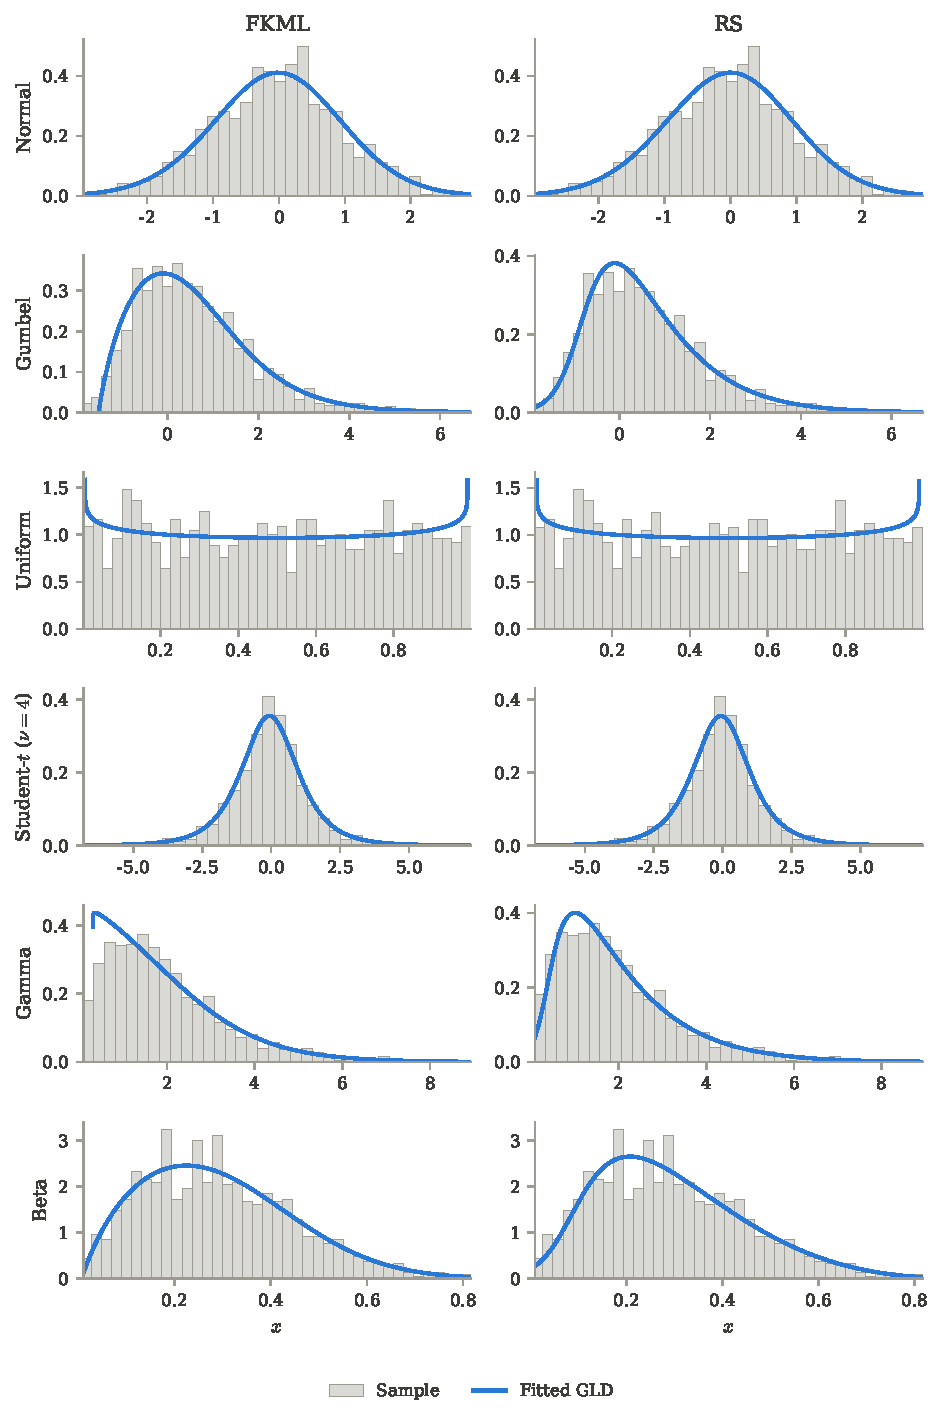
\includegraphics[width=\linewidth,height=0.86\textheight,keepaspectratio]{z_pyglam_fits_en.pdf}
    \caption{GLD fitted by moment matching to the six target distributions
    ($N = 1{,}000$), one row per target and one column per parameterization,
    both fitted to the same sample. The histogram is the sample and the solid line
    the density of the fitted GLD.}
    \label{fig:pyglam_fits}
\end{figure}

\begin{table}[p]
\centering
\caption{Fit quality of the FKML parameterization: medians over 100 independent
replicates per cell, and the interquartile range of the KS distance. Quantile
errors are normalised by the distance between the $P_5$ and the $P_{95}$ of the
target.}
\label{tab:metrics_fkml}
\small
\setlength{\tabcolsep}{4.5pt}
\begin{tabular}{lrrrrrrrr}
\toprule
\textbf{Distribution} & \textbf{$N$} & \textbf{KS} & \textbf{IQR} & \textbf{$D(p\|q)$} &
\textbf{Wass.} & \textbf{$P_5$ (\%)} & \textbf{$P_{50}$ (\%)} & \textbf{$P_{95}$ (\%)} \\
\midrule
Normal & 50 & 0.0562 & 0.0408 & 0.0651 & 0.1307 & 4.48 & 3.14 & 4.74 \\
 & 200 & 0.0320 & 0.0209 & 0.0127 & 0.0742 & 2.84 & 1.54 & 2.57 \\
 & 1,000 & 0.0137 & 0.0086 & 0.0029 & 0.0334 & 0.98 & 0.68 & 1.10 \\
 & 5,000 & 0.0067 & 0.0049 & 0.0015 & 0.0196 & 0.46 & 0.32 & 0.49 \\
\midrule
Gumbel & 50 & 0.0758 & 0.0334 & 0.1196 & 0.2019 & 3.52 & 3.48 & 7.99 \\
 & 200 & 0.0458 & 0.0314 & 0.0482 & 0.0992 & 2.09 & 1.76 & 4.46 \\
 & 1,000 & 0.0220 & 0.0128 & 0.0161 & 0.0512 & 0.87 & 0.73 & 1.91 \\
 & 5,000 & 0.0146 & 0.0059 & 0.0113 & 0.0375 & 0.41 & 0.31 & 0.98 \\
\midrule
Uniform & 50 & 0.0586 & 0.0403 & 0.0132 & 0.0320 & 2.38 & 4.07 & 2.15 \\
 & 200 & 0.0322 & 0.0217 & 0.0043 & 0.0181 & 1.11 & 2.36 & 1.05 \\
 & 1,000 & 0.0172 & 0.0114 & 0.0012 & 0.0102 & 0.54 & 1.21 & 0.61 \\
 & 5,000 & 0.0070 & 0.0033 & 0.0003 & 0.0046 & 0.20 & 0.44 & 0.21 \\
\midrule
Student-$t$ ($\nu=4$) & 50 & 0.0663 & 0.0545 & 0.2102 & 0.2328 & 7.55 & 2.68 & 6.46 \\
 & 200 & 0.0399 & 0.0287 & 0.0392 & 0.1360 & 3.55 & 1.63 & 4.51 \\
 & 1,000 & 0.0193 & 0.0125 & 0.0120 & 0.0750 & 1.73 & 0.93 & 2.33 \\
 & 5,000 & 0.0111 & 0.0073 & 0.0070 & 0.0439 & 1.07 & 0.41 & 1.11 \\
\midrule
Gamma & 50 & 0.0777 & 0.0438 & 0.0630 & 0.2150 & 2.32 & 3.43 & 10.06 \\
 & 200 & 0.0593 & 0.0285 & 0.0241 & 0.1181 & 2.14 & 2.20 & 4.44 \\
 & 1,000 & 0.0374 & 0.0194 & 0.0085 & 0.0605 & 1.44 & 1.09 & 2.37 \\
 & 5,000 & 0.0335 & 0.0122 & 0.0049 & 0.0399 & 1.21 & 0.44 & 0.94 \\
\midrule
Beta & 50 & 0.0679 & 0.0332 & 0.0452 & 0.0221 & 2.64 & 3.85 & 6.71 \\
 & 200 & 0.0329 & 0.0265 & 0.0090 & 0.0120 & 1.22 & 1.85 & 2.87 \\
 & 1,000 & 0.0180 & 0.0106 & 0.0031 & 0.0052 & 0.55 & 1.00 & 1.58 \\
 & 5,000 & 0.0095 & 0.0045 & 0.0014 & 0.0033 & 0.28 & 0.41 & 0.66
\unskip \\
\bottomrule
\end{tabular}
\end{table}

\begin{table}[p]
\centering
\caption{Fit quality of the Ramberg-Schmeiser parameterization, on the same
samples and with the same summaries as Table~\ref{tab:metrics_fkml}.}
\label{tab:metrics_rs}
\small
\setlength{\tabcolsep}{4.5pt}
\begin{tabular}{lrrrrrrrr}
\toprule
\textbf{Distribution} & \textbf{$N$} & \textbf{KS} & \textbf{IQR} & \textbf{$D(p\|q)$} &
\textbf{Wass.} & \textbf{$P_5$ (\%)} & \textbf{$P_{50}$ (\%)} & \textbf{$P_{95}$ (\%)} \\
\midrule
Normal & 50 & 0.0614 & 0.0397 & 0.0398 & 0.1334 & 5.04 & 3.23 & 4.98 \\
 & 200 & 0.0338 & 0.0208 & 0.0110 & 0.0755 & 3.29 & 1.63 & 2.81 \\
 & 1,000 & 0.0143 & 0.0083 & 0.0029 & 0.0346 & 1.06 & 0.66 & 1.01 \\
 & 5,000 & 0.0068 & 0.0052 & 0.0015 & 0.0198 & 0.52 & 0.38 & 0.54 \\
\midrule
Gumbel & 50 & 0.0682 & 0.0346 & 0.0992 & 0.1943 & 2.82 & 3.19 & 8.18 \\
 & 200 & 0.0403 & 0.0287 & 0.0195 & 0.1006 & 1.98 & 1.76 & 4.57 \\
 & 1,000 & 0.0190 & 0.0133 & 0.0052 & 0.0535 & 0.88 & 0.77 & 1.96 \\
 & 5,000 & 0.0122 & 0.0068 & 0.0029 & 0.0341 & 0.68 & 0.41 & 1.32 \\
\midrule
Uniform & 50 & 0.0592 & 0.0392 & 0.0135 & 0.0321 & 2.48 & 4.07 & 2.14 \\
 & 200 & 0.0333 & 0.0227 & 0.0044 & 0.0180 & 1.07 & 2.38 & 1.11 \\
 & 1,000 & 0.0174 & 0.0114 & 0.0013 & 0.0101 & 0.55 & 1.21 & 0.61 \\
 & 5,000 & 0.0070 & 0.0032 & 0.0003 & 0.0046 & 0.21 & 0.42 & 0.21 \\
\midrule
Student-$t$ ($\nu=4$) & 50 & 0.0666 & 0.0559 & 0.1297 & 0.2293 & 7.20 & 2.66 & 6.89 \\
 & 200 & 0.0416 & 0.0300 & 0.0328 & 0.1385 & 4.13 & 1.81 & 4.72 \\
 & 1,000 & 0.0203 & 0.0138 & 0.0117 & 0.0779 & 2.16 & 1.08 & 2.60 \\
 & 5,000 & 0.0131 & 0.0096 & 0.0070 & 0.0466 & 1.32 & 0.52 & 1.27 \\
\midrule
Gamma & 50 & 0.0742 & 0.0432 & 0.0964 & 0.2142 & 2.26 & 2.90 & 10.72 \\
 & 200 & 0.0406 & 0.0200 & 0.0328 & 0.1098 & 1.18 & 1.78 & 5.56 \\
 & 1,000 & 0.0297 & 0.0153 & 0.0251 & 0.0821 & 0.72 & 1.26 & 2.70 \\
 & 5,000 & 0.0261 & 0.0066 & 0.0292 & 0.0858 & 0.62 & 1.45 & 2.51 \\
\midrule
Beta & 50 & 0.0679 & 0.0385 & 0.0411 & 0.0224 & 2.65 & 3.62 & 6.24 \\
 & 200 & 0.0330 & 0.0230 & 0.0112 & 0.0118 & 1.33 & 1.80 & 2.42 \\
 & 1,000 & 0.0185 & 0.0110 & 0.0048 & 0.0059 & 0.88 & 0.92 & 1.35 \\
 & 5,000 & 0.0122 & 0.0056 & 0.0026 & 0.0038 & 0.69 & 0.46 & 0.78
\unskip \\
\bottomrule
\end{tabular}
\end{table}

Both parameterizations recover all six targets to a practically useful accuracy.
At $N = 5{,}000$ the median error at $P_{50}$ is at most $0.44\%$ of the
reference spread under FKML and at most $0.52\%$ under RS on every target but
the Gamma, where it is $1.45\%$; the largest median error anywhere in that row is
$2.51\%$, at the $P_{95}$ of the Gamma under RS. The coefficient of determination
between the estimated densities at $N = 5{,}000$ is at least $0.974$ for every
target except the uniform. There the fitted GLD density turns upward near the two
endpoints while the target is flat, and that comparison is also the one most
affected by the boundary bias of the kernel density estimates; the coefficient
is negative at $N = 50$ and recovers to $0.93$ at $N = 5{,}000$ under both
forms.

On the normal and the uniform the two parameterizations are practically
indistinguishable in every metric. On the Student-$t$ and the Beta, FKML reaches
the smaller KS distance at every $N \geq 1{,}000$. On the Gumbel, RS reaches the
smaller KS distance and divergence at $N = 5{,}000$. On the Gamma the ranking
depends on the metric: RS reaches the smaller KS distance at every
$N \geq 200$, and FKML the smaller divergence, Wasserstein distance and median
error at every $N \geq 1{,}000$.

\subsection{Sampling error or structural error?}\label{subsec:regimes}

The interesting question is not how large the error is but what limits it. The
error of a moment-based fit can be decomposed into a \emph{sampling} component,
from estimating four moments on a finite sample, and a \emph{structural}
component, from the family not containing the target exactly. In simplified form,
\begin{equation}
    E(N) \approx E_{\mathrm{sampling}}(N) + E_{\mathrm{structural}},
    \qquad
    E_{\mathrm{sampling}}(N) \propto N^{-1/2}.
    \label{eq:decomposition}
\end{equation}
The sampling component decreases with $N$, whereas the structural component
remains approximately constant. When the error is dominated by sampling,
\begin{equation}
    \mathrm{KS} \propto N^{-1/2}
    \quad \Longrightarrow \quad
    \log \mathrm{KS} \approx C - \tfrac{1}{2}\log N,
\end{equation}
so regressing the logarithm of the median KS distance on $\log N$ separates the
two regimes. A slope near $-1/2$ with a high coefficient of determination means
the error is predominantly sampling and the fit is as good as the data allows,
whereas a slope near zero means a structural floor dominates and more data will
not help. We label a slope below $-0.45$ as \emph{sampling-limited}, a slope
between $-0.45$ and $-0.30$ as \emph{mixed}, and a flatter one as
\emph{structural floor}. The $95\%$ confidence interval of each slope comes from
$2{,}000$ bootstrap resamples, drawn independently within each sample size.
Table~\ref{tab:rates} reports the regression and
Figure~\ref{fig:pyglam_convergence} shows it.

\begin{table}[htbp]
\centering
\caption{Convergence of the median Kolmogorov-Smirnov distance to the analytical
target: slope of $\log \mathrm{KS}$ against $\log N$ with its bootstrap $95\%$
confidence interval, coefficient of determination, and the regime the slope
implies.}
\label{tab:rates}
\small
\begin{tabular}{llrcrl}
\toprule
\textbf{Param.} & \textbf{Distribution} & \textbf{Slope} & \textbf{95\% CI} &
\textbf{$R^2$} & \textbf{Regime} \\
\midrule
FKML & Normal & $-0.467$ & $[-0.516, -0.436]$ & $0.998$ & sampling-limited \\
 & Gumbel & $-0.367$ & $[-0.387, -0.344]$ & $0.988$ & mixed \\
 & Uniform & $-0.455$ & $[-0.495, -0.409]$ & $0.993$ & sampling-limited \\
 & Student-$t$ ($\nu=4$) & $-0.396$ & $[-0.425, -0.362]$ & $0.997$ & mixed \\
 & Gamma & $-0.193$ & $[-0.228, -0.174]$ & $0.952$ & structural floor \\
 & Beta & $-0.421$ & $[-0.448, -0.394]$ & $0.995$ & mixed \\
RS & Normal & $-0.484$ & $[-0.522, -0.434]$ & $0.999$ & sampling-limited \\
 & Gumbel & $-0.383$ & $[-0.410, -0.354]$ & $0.990$ & mixed \\
 & Uniform & $-0.459$ & $[-0.499, -0.413]$ & $0.993$ & sampling-limited \\
 & Student-$t$ ($\nu=4$) & $-0.363$ & $[-0.400, -0.326]$ & $0.992$ & mixed \\
 & Gamma & $-0.221$ & $[-0.239, -0.192]$ & $0.893$ & structural floor \\
 & Beta & $-0.369$ & $[-0.392, -0.338]$ & $0.977$ & mixed
\unskip \\
\bottomrule
\end{tabular}
\end{table}

\begin{figure}[p]
    \centering
    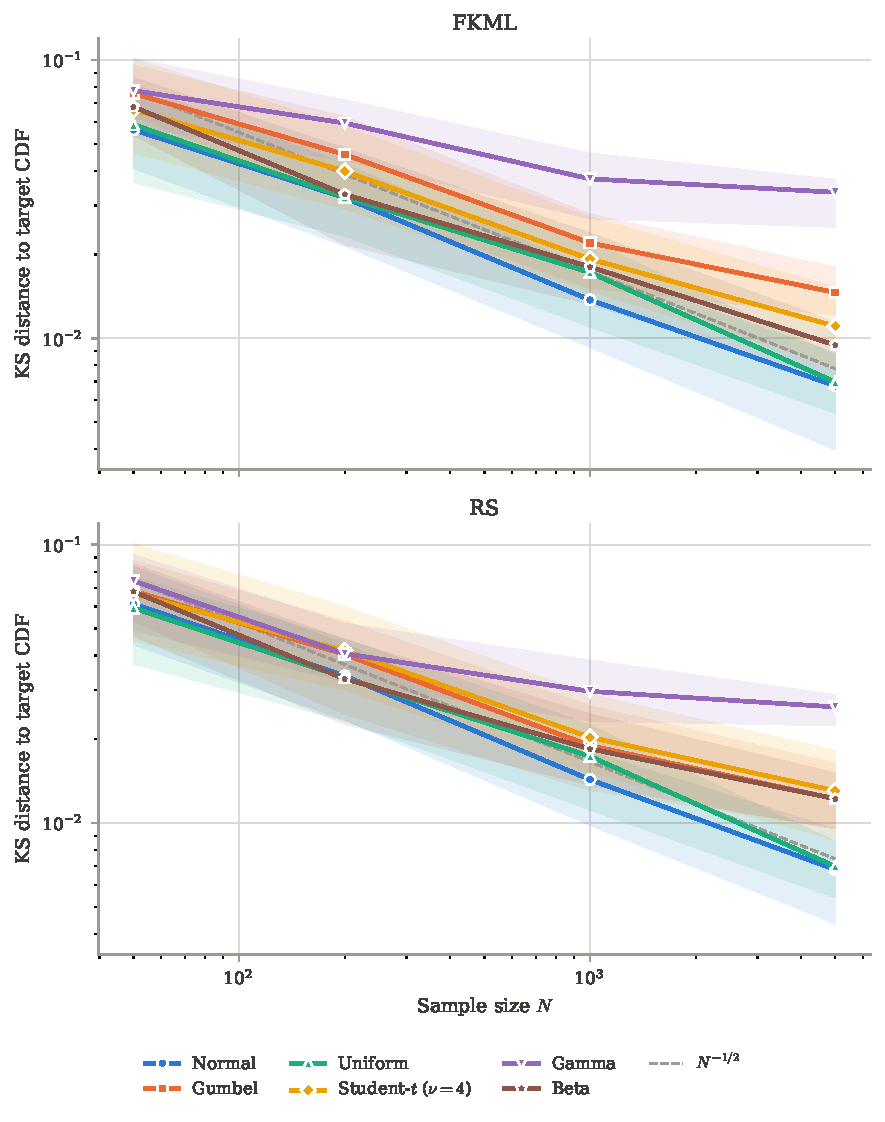
\includegraphics[width=\linewidth,height=0.86\textheight,keepaspectratio]{z_pyglam_convergence_en.pdf}
    \caption{Convergence of the Kolmogorov-Smirnov distance between the fitted
    GLD and the analytical target, against sample size, one panel per
    parameterization. Logarithmic axes; each point is the median of 100
    independent replicates and the band their interquartile range. The dashed
    guide has slope $-1/2$, the theoretical sampling rate.}
    \label{fig:pyglam_convergence}
\end{figure}

For the normal and the uniform the two parameterizations behave identically and
converge close to the theoretical rate, with slopes between $-0.484$ and $-0.455$
and $R^2 \geq 0.993$. There is no detectable structural component: the GLD
represents a symmetric unbounded target and a bounded one with the precision the
data allows, and the choice of parameterization is immaterial.

The Beta and the Gumbel fall in the mixed regime under both forms, a small
structural component that slows the decay without stopping it. On the Gumbel the
two confidence intervals overlap, $[-0.387, -0.344]$ under FKML and
$[-0.410, -0.354]$ under RS, and the rates cannot be told apart. The fitted
parameters show that the two forms reach the exponential right tail of the
Gumbel in different ways. In the FKML form an exponential tail is the
logarithmic case $\lambda_4 = 0$ of Equation~\eqref{eq:qfkml}, and the fits
settle near it, at a median $\lambda_4 = -0.024$ at $N = 5{,}000$. The RS form
has no logarithmic case: it can only approach an exponential tail as the limit
in which $\lambda_2$, $\lambda_3$ and $\lambda_4$ vanish together while their
ratios stay finite, and that is where its fits go, with all three medians within
$0.04$ of zero. The limit is the common edge of the region with positive shapes
and the region with negative shapes, and the fits land on both sides of it: at
$N = 5{,}000$, $14\%$ of them have $\lambda_2 < 0$, with a median KS distance of
$0.0178$ against $0.0119$ for the others.

The Gamma is the one target with a structural floor under both forms, with
slopes of $-0.193$ (FKML) and $-0.221$ (RS). Its density rises linearly from zero
at the left endpoint, which neither moment-matched GLD reproduces. The FKML fit,
at a median $\lambda_3 = 0.94$ and $\lambda_4 = -0.005$, rises almost vertically
at that endpoint (Figure~\ref{fig:pyglam_fits}), and its median KS distance stops
at $0.034$. The RS fit takes a strongly asymmetric shape, with a median
$\lambda_3 = 31$ and $\lambda_4 = 0.63$, whose density at the left endpoint is
finite and positive; its median KS distance stops at $0.026$, at the price of
the larger divergence and median error noted above. Both fits reproduce the same
four sample moments, and they differ in which part of the distribution they get
wrong, which is the case for scoring every fit with the diagnostics of
Section~\ref{sec:software} rather than trusting the moment match alone.

The Student-$t$ shows a mixed regime under both forms, with slopes of $-0.396$
under FKML and $-0.363$ under RS. Here the limitation is not the family but the
estimator. Because the kurtosis of the target is infinite, the sample kurtosis
does not converge: over the replicates of the study its median grows from $4.1$
at $N = 50$ to $10.2$ at $N = 5{,}000$. The moments being matched therefore move
with $N$, and the fitted shapes follow them towards the pole of the fourth
moment: the median $\lambda_3$ goes from $-0.02$ at $N = 200$ to $-0.14$ at
$N = 5{,}000$ under FKML, and from $-0.06$ to $-0.14$ under RS. With both shapes negative the fitted
distributions are unbounded on both sides, as the target is, but moment matching
cannot settle on a limit, and the convergence slows accordingly.

Three consequences follow. First, whether a structural component appears depends
on the target: none for the normal and the uniform, a small one for the Gumbel
and the Beta, a floor for the Gamma. Second, where the parameterizations differ,
the difference is not always in the rate but in the shape of the error: on the
Gamma the two forms match the same moments with distributions that fail in
different places, and on the Gumbel a share of the RS fits falls on the wrong
side of a degenerate limit, which a study of one parameterization, or of mean errors
alone, would not reveal. Third, the regime decomposition also diagnoses
the estimator, as the Student-$t$ shows: a target at the edge of the moment
domain slows moment matching under either form, and the remedy there is a
different estimator rather than a different parameterization.

The classical test behaves as its power dictates. At the $5\%$ level, the
rejection rate of the Kolmogorov-Smirnov test at size $N$ stays between $3\%$ and
$9\%$ for the normal at every sample size, consistent with the nominal level. On
the targets with a structural component it grows with $N$ while the fit itself
improves: at $N = 5{,}000$ it reaches $26\%$ (FKML) and $35\%$ (RS) on the Gumbel,
$24\%$ and $29\%$ on the Student-$t$, and $76\%$ and $74\%$ on the Gamma. The
apparent paradox is only the test gaining power: with more data it detects a
residual discrepancy that remains small in magnitude.

\subsection{Validity and cost of the fits}\label{subsec:validity_results}

Section~\ref{subsec:validity} showed that validity is a sign condition on
$\lambda_2$ under FKML and a region condition under RS, and
Section~\ref{sec:software} described how the estimator enforces both.
Table~\ref{tab:validity} reports the result, together with the fitting time.

\begin{table}[htbp]
\centering
\caption{Validity and cost of the fits, over 400 fits per cell.
\emph{Candidates} is the share of the 15 multi-start candidates whose quantile
function is finite and non-decreasing; \emph{selected} is the share of the fits
returned by the estimator that are distributions. The optimizer reported
convergence for every fit. Times are per fit, in seconds.}
\label{tab:validity}
\small
\begin{tabular}{llrrrrr}
\toprule
& & & \multicolumn{2}{c}{\textbf{Valid (\%)}} & \multicolumn{2}{c}{\textbf{Time (s)}} \\
\cmidrule(lr){4-5} \cmidrule(lr){6-7}
\textbf{Param.} & \textbf{Distribution} & \textbf{Fits} &
\textbf{Candidates} & \textbf{Selected} & \textbf{Mean} & \textbf{SD} \\
\midrule
FKML & Normal & 400 & 100.0 & 100.0 & 0.19 & 0.34 \\
 & Gumbel & 400 & 100.0 & 100.0 & 0.16 & 0.11 \\
 & Uniform & 400 & 99.6 & 100.0 & 2.29 & 2.01 \\
 & Student-$t$ ($\nu=4$) & 400 & 100.0 & 100.0 & 0.20 & 0.13 \\
 & Gamma & 400 & 100.0 & 100.0 & 0.33 & 0.44 \\
 & Beta & 400 & 100.0 & 100.0 & 0.26 & 0.58 \\
RS & Normal & 400 & 100.0 & 100.0 & 0.20 & 0.11 \\
 & Gumbel & 400 & 100.0 & 100.0 & 0.30 & 0.14 \\
 & Uniform & 400 & 100.0 & 100.0 & 0.26 & 0.12 \\
 & Student-$t$ ($\nu=4$) & 400 & 100.0 & 100.0 & 0.28 & 0.14 \\
 & Gamma & 400 & 100.0 & 100.0 & 0.30 & 0.13 \\
 & Beta & 400 & 100.0 & 100.0 & 0.32 & 0.22
\unskip \\
\bottomrule
\end{tabular}
\end{table}

Every selected fit is a distribution. Under RS every candidate is one as well,
because the admissible regions are imposed inside the residual function and the
solver never leaves them. Under FKML the objective does not constrain the sign of
$\lambda_2$, and $29$ of the $36{,}000$ candidates were not distributions, $28$ of
them because they ended with $\lambda_2 < 0$: parameter vectors that reproduce
the four sample moments and are reported as converged by the optimizer, yet whose
quantile function is decreasing. Most of them, $24$, occur on the uniform. The
screens of
Section~\ref{sec:software} exclude them before selection. The general point is
that optimizer convergence says nothing about validity: the moment equations
admit such roots, and only an explicit check keeps them out of the result.

A fit takes $0.28$ seconds on average under RS, with little dispersion, and
$0.57$ seconds under FKML, with a median of $0.18$ seconds and a long right tail
driven by the uniform target, where a fit takes $2.29$ seconds on average. These
times were measured inside $31$ worker processes running in parallel on a
$32$-thread workstation, and the whole study, including the scoring of every
fit, took about seven minutes of wall time.

\subsection{Comparison with the R implementations}\label{subsec:r_comparison}

The implementation was cross-validated against the R packages \texttt{gld}
\parencite{KingGld} and \texttt{GLDEX} \parencite{Su2007JSS, SuGLDEX}, running on
R 4.6.1 \parencite{RCore}, in two parts.

The first part compares the functions themselves. For six parameter vectors of
each parameterization, spanning the fits of this study, asymmetric and
heavy-tailed shapes, and, for RS, the regions with positive, negative and mixed
signs, the quantile function, the CDF and the density of \texttt{pyGLAM} were
evaluated on $199$ probabilities and compared with \texttt{qgl}, \texttt{pgl} and
\texttt{dgl} of \texttt{gld}, and the first four moments with
\texttt{fun.theo.mv.gld} of \texttt{GLDEX}. Table~\ref{tab:r_functions} reports
the largest discrepancy. The quantile functions agree to rounding error and the
moments to $10^{-9}$ or better; the CDF and the density agree to $10^{-8}$, the
tolerance of the numerical inversion of the quantile function.

\begin{table}[htbp]
\centering
\caption{Largest discrepancy between \texttt{pyGLAM} and the R packages over six
parameter vectors per parameterization: quantile relative to the range of the
evaluated quantiles, CDF in probability, density relative to its maximum, mean in
standard deviations, variance relatively, skewness and kurtosis in absolute
terms.}
\label{tab:r_functions}
\footnotesize
\setlength{\tabcolsep}{3.5pt}
\begin{tabular}{lrccccccc}
\toprule
\textbf{Param.} & \textbf{Sets} & \textbf{Quantile} & \textbf{CDF} & \textbf{Density} &
\textbf{Mean} & \textbf{Variance} & \textbf{Skewness} & \textbf{Kurtosis} \\
\midrule
FKML & 6 & $2.0 \times 10^{-15}$ & $1.0 \times 10^{-8}$ & $1.2 \times 10^{-8}$ & $5.4 \times 10^{-16}$ & $5.7 \times 10^{-15}$ & $7.1 \times 10^{-14}$ & $1.5 \times 10^{-12}$ \\
RS & 6 & $1.4 \times 10^{-15}$ & $1.0 \times 10^{-8}$ & $1.5 \times 10^{-8}$ & $2.3 \times 10^{-15}$ & $8.0 \times 10^{-15}$ & $2.0 \times 10^{-13}$ & $5.1 \times 10^{-10}$
\unskip \\
\bottomrule
\end{tabular}
\end{table}

The second part compares the fits. Fifty samples of each target at
$N = 1{,}000$ and $N = 5{,}000$ were fitted by moment matching with
\texttt{pyGLAM} and with \texttt{fun.RMFMKL.mm} and \texttt{fun.RPRS.mm} of
\texttt{GLDEX}, and every fit was scored by the same code. Because the moment
equations have several roots, the parameters are not expected to coincide; the
comparison is on the fitted distributions, and Table~\ref{tab:r_fits} reports
the KS distance and the Wasserstein distance to the analytical target, the
latter normalised by the distance between the $P_5$ and the $P_{95}$ of the
target, together with the largest gap between the two fitted quantile functions
on $[0.01, 0.99]$, in the same units. All $2{,}400$ fits of both packages were
valid distributions.

\begin{table}[htbp]
\centering
\caption{Fits of the same samples by \texttt{pyGLAM} (py) and \texttt{GLDEX} (R):
share of valid fits, medians over 50 samples of the KS distance and of the
normalised Wasserstein distance to the target, and median of the largest gap
between the two fitted quantile functions.}
\label{tab:r_fits}
\footnotesize
\setlength{\tabcolsep}{3.5pt}
\begin{tabular}{llrrrrrrrr}
\toprule
& & & \multicolumn{2}{c}{\textbf{Valid (\%)}} & \multicolumn{2}{c}{\textbf{KS}} &
\multicolumn{2}{c}{\textbf{Wasserstein}} & \textbf{Quantile} \\
\cmidrule(lr){4-5} \cmidrule(lr){6-7} \cmidrule(lr){8-9}
\textbf{Param.} & \textbf{Distribution} & \textbf{$N$} & \textbf{py} & \textbf{R} &
\textbf{py} & \textbf{R} & \textbf{py} & \textbf{R} & \textbf{gap} \\
\midrule
FKML & Normal & 1,000 & 100 & 100 & 0.0124 & 0.0124 & 0.0090 & 0.0090 & 0.0000 \\
 &  & 5,000 & 100 & 100 & 0.0057 & 0.0057 & 0.0041 & 0.0041 & 0.0000 \\
 & Gumbel & 1,000 & 100 & 100 & 0.0261 & 0.0230 & 0.0154 & 0.0143 & 0.0609 \\
 &  & 5,000 & 100 & 100 & 0.0146 & 0.0187 & 0.0078 & 0.0099 & 0.0640 \\
 & Uniform & 1,000 & 100 & 100 & 0.0142 & 0.0150 & 0.0086 & 0.0100 & 0.0036 \\
 &  & 5,000 & 100 & 100 & 0.0067 & 0.0076 & 0.0037 & 0.0043 & 0.0021 \\
 & Student-$t$ ($\nu=4$) & 1,000 & 100 & 100 & 0.0180 & 0.0180 & 0.0148 & 0.0148 & 0.0000 \\
 &  & 5,000 & 100 & 100 & 0.0101 & 0.0101 & 0.0090 & 0.0090 & 0.0000 \\
 & Gamma & 1,000 & 100 & 100 & 0.0413 & 0.0250 & 0.0141 & 0.0131 & 0.0516 \\
 &  & 5,000 & 100 & 100 & 0.0313 & 0.0243 & 0.0083 & 0.0098 & 0.0461 \\
 & Beta & 1,000 & 100 & 100 & 0.0171 & 0.0290 & 0.0100 & 0.0187 & 0.0413 \\
 &  & 5,000 & 100 & 100 & 0.0096 & 0.0283 & 0.0048 & 0.0173 & 0.0422 \\
\midrule
RS & Normal & 1,000 & 100 & 100 & 0.0138 & 0.0138 & 0.0094 & 0.0094 & 0.0000 \\
 &  & 5,000 & 100 & 100 & 0.0060 & 0.0060 & 0.0040 & 0.0040 & 0.0000 \\
 & Gumbel & 1,000 & 100 & 100 & 0.0200 & 0.0302 & 0.0135 & 0.0197 & 0.0443 \\
 &  & 5,000 & 100 & 100 & 0.0110 & 0.0121 & 0.0063 & 0.0068 & 0.0000 \\
 & Uniform & 1,000 & 100 & 100 & 0.0144 & 0.0149 & 0.0086 & 0.0097 & 0.0038 \\
 &  & 5,000 & 100 & 100 & 0.0067 & 0.0076 & 0.0037 & 0.0047 & 0.0024 \\
 & Student-$t$ ($\nu=4$) & 1,000 & 100 & 100 & 0.0195 & 0.0272 & 0.0160 & 0.0190 & 0.0000 \\
 &  & 5,000 & 100 & 100 & 0.0122 & 0.0122 & 0.0101 & 0.0101 & 0.0000 \\
 & Gamma & 1,000 & 100 & 100 & 0.0292 & 0.0252 & 0.0192 & 0.0147 & 0.1197 \\
 &  & 5,000 & 100 & 100 & 0.0275 & 0.0153 & 0.0192 & 0.0083 & 0.1238 \\
 & Beta & 1,000 & 100 & 100 & 0.0176 & 0.0180 & 0.0109 & 0.0113 & 0.0000 \\
 &  & 5,000 & 100 & 100 & 0.0111 & 0.0124 & 0.0062 & 0.0071 & 0.0000
\unskip \\
\bottomrule
\end{tabular}
\end{table}

On the normal and the Student-$t$ the two packages return the same distribution
under both parameterizations, with a quantile gap below $10^{-4}$, and so they
do for the RS fits of the Beta and, at $N = 5{,}000$, of the Gumbel. On the
uniform the gaps stay below $0.004$. Elsewhere the two packages land on different
solutions, for two different reasons. Under FKML, \texttt{pyGLAM} reproduces the
sample moments to the precision of the solver, whereas \texttt{GLDEX} stops at a
median moment discrepancy of $0.08$ to $0.10$ on the Gumbel, the Gamma and the
Beta. The inexact solution is not always the worse one: it is farther from the
target on the Beta, with a median KS distance of $0.028$ against $0.010$ at
$N = 5{,}000$, but closer on the Gamma, with $0.024$ against $0.031$, another
instance of a closer moment match not being a closer distribution. Under RS,
both packages reproduce the moments of the Gamma, but at different roots: the
dense search of \texttt{GLDEX}, over $10{,}000$ quasi-random starting points,
reaches one with a median KS distance of $0.015$, whereas the $15$ starts of
\texttt{pyGLAM} reach $0.027$, and the full grid of $29$ starts $0.025$.

\texttt{pyGLAM} is also faster. Measured under the same conditions, with one
process per core, a fit takes a median of $0.17$ seconds under FKML and $0.18$
under RS, against $1.09$ and $4.92$ seconds for \texttt{GLDEX}.
